\documentclass{article}
\usepackage[parfill]{parskip}
\usepackage{graphicx}
\usepackage{float}
\usepackage{placeins}
\usepackage[top=2 cm, bottom=2 cm, left=2 cm, right=2 cm]{geometry}
\usepackage{amsmath}

\usepackage[
    backend=biber,
    style=alphabetic,
    sorting=none
]{biblatex}
\addbibresource{bibliography.bib}

\title{Modeling project: DNA packaging in a virus}
\author{}
\date{}

\begin{document}

\maketitle

\begin{abstract}
\noindent
In order to infect a host cell, bacteriophage viruses must eject their genome, which is then replicated, followed by the synthesis of the proteins encoded in it. Once the concentration of the proteins is high enough, the construction of the viral capsids, which are rigid\footnote{They will  be modelized as rigid in our approach, eventhough it is not actually the case} protein boxes, is initiated. The next step is the packaging of the viral DNA inside the capsids, which can then be injected into other host cells. The packaging of DNA in these viruses is thus an essential step in their life cycle. In this article, we describe a simple physical model explaining this packaging process for diversely shaped capsids. 
\end{abstract}


\section{Introduction}
The dynamics of the packing of double-stranded DNA in bacteriophages and other viruses using the same mechanism (ATP-dependent packaging of the DNA into a preformed capsid) has been investigated both experimentally and theoretically. There are two main types of theoretical models: thermodynamic quasi-static models which considers DNA as a polymer (see \cite{phillips2005}) and molecular dynamics models which simulate it as a series of beads connected by springs (see \cite{Petrov2008}). These two approaches lead to different predictions and there is still a debate about the nature of the dynamics and the forces involved in the mechanism.\cite{Berndsen2014} The physical model we present is of the former type. It assumes that DNA takes a single conformation inside the capsid and organizes itself as a spool. However, the first experimental measurement of the spatial organization of DNA inside the capsid during the packing process has been observed only in 2008 by Comoli and al. \cite{comoli2008}. They showed that contrarily to what was believed before (for instance in \cite{phillips2005, purohit2003}), DNA tends to organize itself in the spool structure very late in the packaging process. Indeed, until $78\%$ of the genome is packed, the DNA inside the capsid stays in a disordered phase. We can see that the dynamics of DNA packing inside viruses is still an active subject of research. The table below contains some order of magnitudes for quantities of interest for visualization purposes.

\begin{table}[h]
    \centering
    \begin{tabular}{|| r | c | c | l ||}
        \hline \hline
        \textbf{Name of the variable} & \textbf{Symbol} & \textbf{Value} & \textbf{Source} \\
        \hline \hline
        Diameter of the capsid  & $R_{out}$   & $21~to~ 54~nm$ & Phage $\phi29$ \cite{tao1998}  \\
        Diameter of the DNA    & $ d_{dna}$  & $1~nm$           & \cite{phillips2005} \\
        Length of the DNA strand & $ L_{tot}$  & $5.5\times10^{3}~nm$  & Phage $\phi29$ \cite{tao1998} \\
        Persistence length       & $ \xi_p $   & $50~nm$           & \cite{smith2001} \\
        Packing force              & $ F_{pack}$  & $10~pN$          & \cite{phillips2005} \\
        \hline \hline
    \end{tabular}
    \caption{Some order of magnitudes about DNA in a viral capsid}
    \label{tab:figures}
\end{table}
The article is structured as follows: the next section introduces the physical model for the packaging of DNA inside a viral capsid. The following derives the expression for the force resisting the packaging for three different geometries and includes a numerical and qualitative analysis of the results. The final section concludes with final remarks about the model's predictions and how it could be improved.

\section{Simple physical model of DNA packaging inside a viral capsid}

The goal of this section is to develop a physical model that will allow us to compute the force produced by the motor during packing. 
In our model, we make the assumption that only the DNA strands participate in the packaging and the capsid is assimilated to an infinitely rigid vessel of radius $ R_{out}$\footnote{We only consider capsids that are invariant under rotation and are cylindrical, cylindrical or caped-cylindrical (see figure \ref{fig:shapes}}. Moreover, we assume that DNA is a polymer, which is charged since DNA is strongly negative. As a starting point, we use the worm-like chain model for semi-flexible polymers, which can be built from simple physical arguments and used to construct mathematical expressions that are useful to understand the bending of DNA during the packing mechanism. To this model, we then add a term accounting for the interactions between the DNA strands. As DNA is solvated in solution, the nature of the interactions between the strands will depend on the type of the surrounding ions. In particular, we only consider fully repulsive conditions.

\subsection{Building the Hamiltonian of the worm-like chain model}
The only element we want to keep in our model is the stiffness of the polymer, which is represented by a binding energy, and the repulsion between two points of the polymer. We do not include tension in our model because the extremity of the polymer is free and any tension will relax very fast (this is an assumption). We define the curvilinear coordinate along the DNA strand $s$, the 'trajectory'/ 'parametrized curve' representing the strand $r(s)$, and $\kappa$ which is a kernel that represents the energy of interaction between two bits of unit length $s, s+ds$ at two distinct points along the strand.

Then, keeping only the lowest order terms in the Hamiltonian, we end up with the following form:
\begin{eqnarray*}
    G &=& \int_{0}^{L} ds \left[ \frac{k_B T \xi_p}{2} \left( \partial_s^2 \vec{r}(s) \right)^2 + \int_0^L ds^\prime \kappa \left(\vec{r}(s), \vec{r}(s^\prime) \right) \right]
\end{eqnarray*}
 where $k_B$ is the Boltzman constant, $T$ the temperature \footnote{T = 300K for instance}, and $\xi_p$ the persistence length of the polymer \footnote{This typically means that if we define as $\vec{t}$ the tangent vector of the polymer at $s$ and $\vec{t^\prime}$ the tangent vector of the polymer at $ s^\prime $, we typically have $\left\langle \vec{t} . \vec{t}^\prime \right\rangle \propto \frac{k_B T}{2} \exp{ \left( \frac{\left\vert s-s^\prime\right\vert }{\xi_p} \right )}$ where $\left\langle \dots \right\rangle $ is an average over the configurations of the polymer}.
We see that the term in $ \left( \vec{r}(s) \right)^2 $ will correspond to bending. The other terms can allow to implement any kind of two point interaction of the DNA strand.

\subsection{Building the two terms $G_{bend}$ and $G_{int}$}
The goal of this subsection is to write the two terms we have identified in the Hamiltonian in a more explicit form.

\subsubsection{Expression of the bending force}
To put the bending force in a nice expression, we start from the empirical observation of DNA packed inside the capsid. The DNA is packed as a spool. So we will assume that it is always so. This leads to the assumption that the radius of bending is almost constant: $\left( \partial_s^2 \vec{r} \right)^2=\frac{1}{R^2}$. We transform the integral of the curvilinear coordinate into an integral over the radial coordinate of the piece of strand in the spool:

\begin{eqnarray*}
    \int_{0}^{L} ds = \int_{R_{int}} ^{R_{out}} \rho (R) dR \int_0^{2\pi} R d \theta 
\end{eqnarray*}

Where $R_{int}$ is the internal radius of the spool, $R_{out}$ is the outer radius of the spool (which is the same as the radius of the capsid), and $\rho$ is the density of hoops of radius $R$. This density gives the number of hoops with radius in between $R$ and $R+ dR$. If we denote as $N(R)$ the number of circles of DNA that can be at radius $R$, we have $\rho (R) = \frac{N(R)}{\frac{\sqrt{3}}{2} d_s } $ because in the horizontal direction, there is one layer every $\frac{\sqrt{3} d_s}{2}$. In the vertical direction, one can relate $N(R)$ to the shape  of the capsid. We define $h(R)$ as the height of a column of hoops at radius $R$. We thus have $N(R) = \frac{h(R)}{d_s} $ because in the vertical direction, there is one strand every $d_s$ (see figure \ref{fig:hexagone}).

\begin{figure}[H]
    \centering
    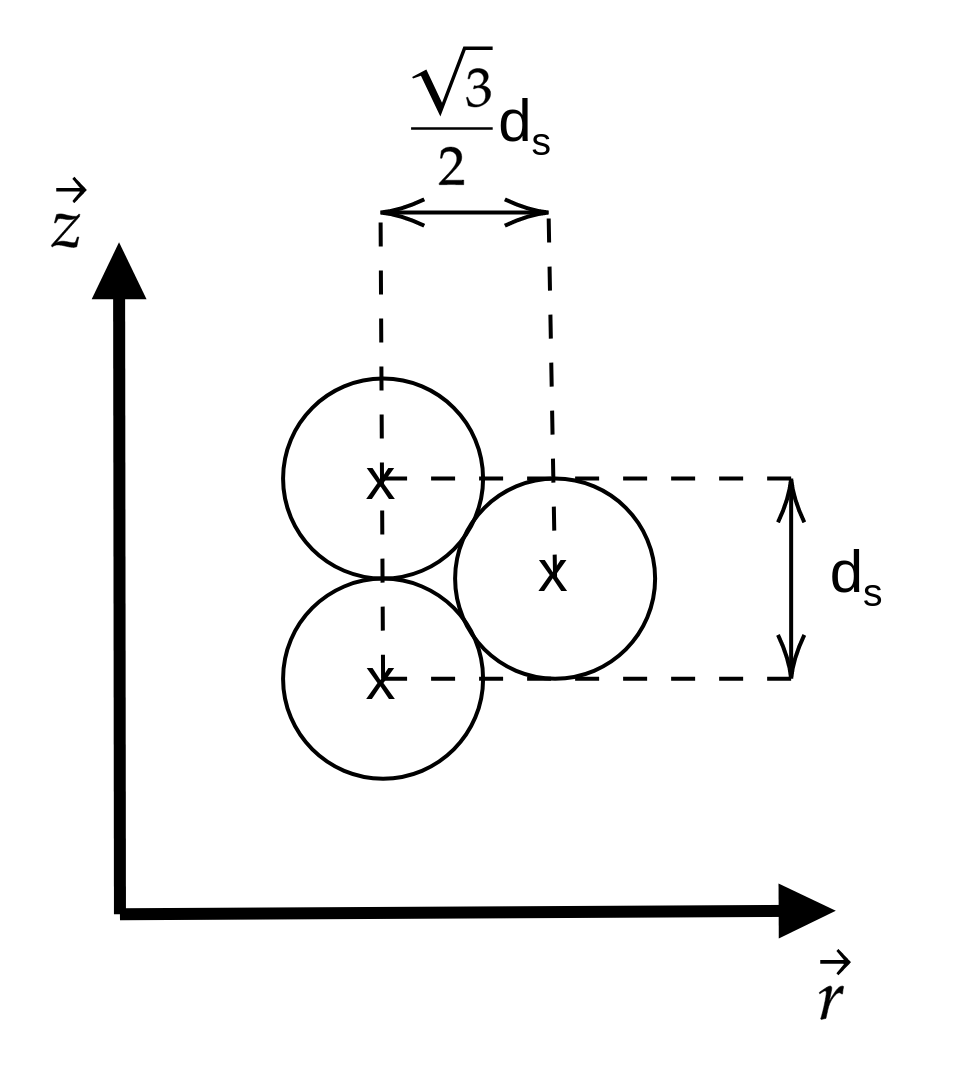
\includegraphics[height=0.3\textwidth]{schema_packing.png}
    \caption{Schematic of the packing of DNA strands.}
    \label{fig:hexagone}
\end{figure}

Putting all these expressions together, we obtain bending energy:
\begin{eqnarray}
    G_{bend} &=& \frac{2 \pi \xi_p k_B T}{\sqrt{3} d_s^2} \int_{R_{int}}^{R_{out}} \frac{h(R)}{R} dR
\end{eqnarray}

We see that the bending term takes into account the rigidity of the polymer and the shape of the capsid. The latter will be encoded in the $h$ function. We come back to the computations for different shapes later, for now let us look at the repulsion term.

\subsubsection{DNA-DNA repulsion}

The other term that must be taken into account in the energy of the system is the repulsion between DNA strands. In fact, each base pair is charged with a charge $-2$ \cite{alberts2002} and DNA is a strongly charged molecule $ \sim - 7 C.nm^{-1} $. Due to this charge, DNA could not be stable if it was not in a solution containing counter ions \cite{singh2015}. In this model we will only consider interaction between nearest neighbours. Once again this choice is based on the assumption that the spool is always very well organized.

The force has been determined experimentally based on measurements of osmotic pressure. The force per unit length between two neighbouring DNA strands separated by a distance $d_s$ is : $f_{el} \left(d_s\right) = \frac{F_0 d_s}{\sqrt{3}} exp \left(\frac{-d_s}{c}\right) $, where $F_0$ is homogeneous to a force per unit length and $c$ to a length. These are parameters that should be determined from fits on experimental data. The form of this expression comes from the fact that the ions in the solution tend to screen the charge of the DNA strands. That is why we do not have a behaviour in $\frac{1}{d_s^2}$ as one might expect for Coulomb repulsion. No direct measurement of $F_0$ and $c$ have been done to our knowledge. \cite{purohit2003} To compute the potential energy of interaction per unit length of two strands, we have to compute the work needed to bring two strands that are separated by an infinite distance to a distance of $d_s$ between them. By doing so, we compute the energy of one link between two DNA strands:

\begin{eqnarray*}
    G_{el}^{link} &=& \int_{\infty}^{d_s} f_{el} \left( d'_s \right) dd'_s \\
    & = & \int_{\infty}^{d_s} \frac{F_0 d'_s}{\sqrt{3}} exp \left(\frac{-d'_s}{c}\right) dd'_s \\
    & = & \frac{F_0}{\sqrt{3}} \left( c^2 + cd_s \right) exp \left( \frac{- d_s}{c} \right) \;\; \textnormal{(we made an intergration by part)} \label{eq:gelec}
\end{eqnarray*}

Since each strand has six neighbours, we have to multiply by a factor $\frac{6}{2} = 3$ to avoid double-counting each link (see figure \ref{fig:lattice}). We then have to multiply this energy per unit length by the full length of the DNA strand:
\begin{eqnarray}
    G_{charge} &=& 3 L G_{el}\left(ds\right) = L\sqrt{3} F_0 \left( c^2 + cd_s \right) exp \left( \frac{- d_s}{c} \right) \label{eq:gcharge}
\end{eqnarray}

\begin{figure}[H]
    \centering
    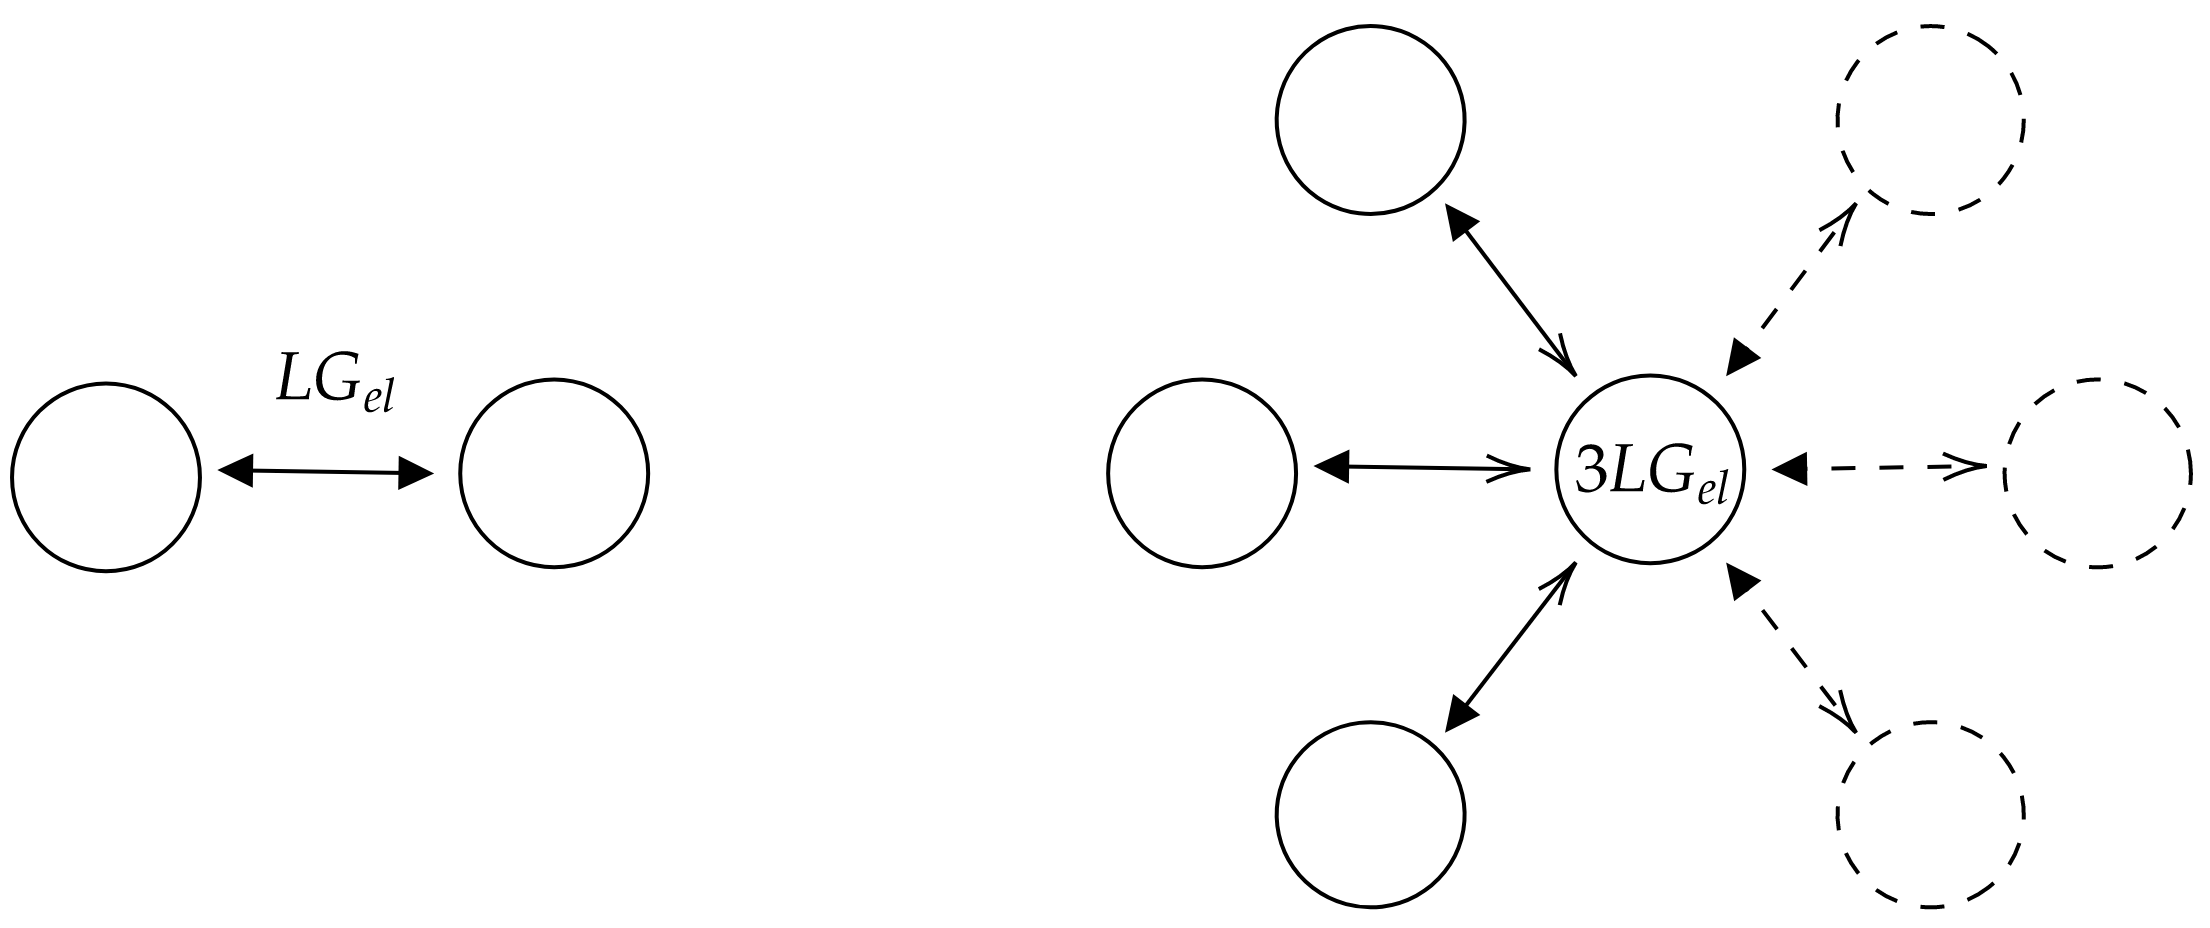
\includegraphics[width=0.5\textwidth]{diagram_Gcharge.png}
    \caption{Repulsion between DNA strand.}
    \label{fig:lattice}
\end{figure}

The expression might seem very simple. In fact, it also contain a dependence in the geometry of the capsid through $L$. The length of DNA in the capsid is the following (see the appendix equation \ref{eq:Ldef}):

\begin{eqnarray*}
    L & = & \frac{4 \pi}{\sqrt{3} d_s^2} \int_{R_{int}}^{R_{out}} R h(R) dR
\end{eqnarray*}

We have derived the explicit expression for each term in the Hamiltonian. In the next subsection, we put everything together and minimize the Hamiltonian. 
\subsection{The equation on $d_s$}

In this section we are going to minimize analytically the expression of $G$. This approach relies on the fact that, at mechanical equilibrium, the DNA strands are arranged in the configuration which minimizes the energy. As the length of DNA inside the capsid is fixed, the only parameter that can be optimized is $d_s$. Let us write the full expression of $G$:

\begin{eqnarray}
    G_{tot} &=& \frac{2 \pi \xi_p k_B T}{\sqrt{3} d_s^2} \int_{R_{int}}^{R_{out}} dR \frac{h(R)}{R} + L \sqrt{3} F_0 \left( c^2 +cd_s \right) \exp{ \left( \frac{d_s}{c} \right) }
    \label{eq:Gtot}
\end{eqnarray}

Writing the condition $ \frac{\partial G_{tot}}{\partial d_s} = 0 $ under the constraint that $L$ is fixed leads to the equation (see the appendix for details):
\begin{eqnarray}
    \sqrt{3} F_0 \exp{ \left( \frac{-d_s}{c} \right) } &=& \frac{\xi_p k_B T}{d_s^2 R_{int}^2} - \frac{\xi_p k_B T}{d_s^2} \frac{\int_{R_{int}}^{R_{out}} \frac{h(R)}{R} dR}{\int_{R_{int}}^{R_{out}} R h(R) dR} 
    \label{eq:deriv_ds_final}
\end{eqnarray}

We see that this is a closed hierarchy and that it can in principle be solved. However, analytical solving for each length does not seem to be at hand \cite{purohit2003}. We thus rely on numerically solving this equation.

\subsection{The force during packing}
Now let us imagine that we have found the value $d^*_s$ that minimizes the free energy. We can reintroduce it in $G$ and deduce the force the motor needs to generate via $F_{pack} = \frac{\partial G}{\partial L}$. We deduce from equation (\ref{eq:Gtot}) that (see appendix \emph{Computation of the force} for detailed derivation):
\begin{eqnarray}
    F_{pack} &=& \frac{\xi_p k_B T}{2 R_{int}^2} + F_0 \sqrt{3} \left( c^2 + c d_s^* \right) \exp{ \left( \frac{-d^*_s}{c} \right) }
    \label{eq:F}
\end{eqnarray}

This is exactly the expression that have been given in \cite{purohit2003} (see equation [19] of the reference).
As a conclusion, we have seen how to derive the expression for the force of the motor. Now we want to find a more explicit form for this force. We would like to express it as a function of the percentage of DNA packed inside the capsid. We will see in the next section that for that we need to specialize to a given geometry of capsid.

\section{Computing of the force in various geometries}

In this section we will show that for a typical geometry of capsid, we can express the force as a fucntion of the percentage of DNA packed inside the capsid, the radius $R_{out}$ and the packing density $\rho_{pack} = \frac{\Omega_{dna}}{\Omega_{caps}}$ (it the ratio of the volume occupied by the DNA when it is fully packed divided by the volume of the capsid). We remark here that $ \Omega_{dna} = \frac{\sqrt{3}d_s^2}{2} L$. It is interesting to use these three parameters as they correspond to quantities that are easy to access experimentally. \cite{phillips2005, purohit2003} We will distinguish three geometry of capsid : (1) \emph{cylindrical} when the capsid is a cylinder, (2) \emph{spherical} when the capsid is a sphere, and (3) \emph{capped cylinder} when the capsid is a cylinder capped with two hemispheres (see figure \ref{fig:shapes}).

\begin{figure}[H]
    \centering
    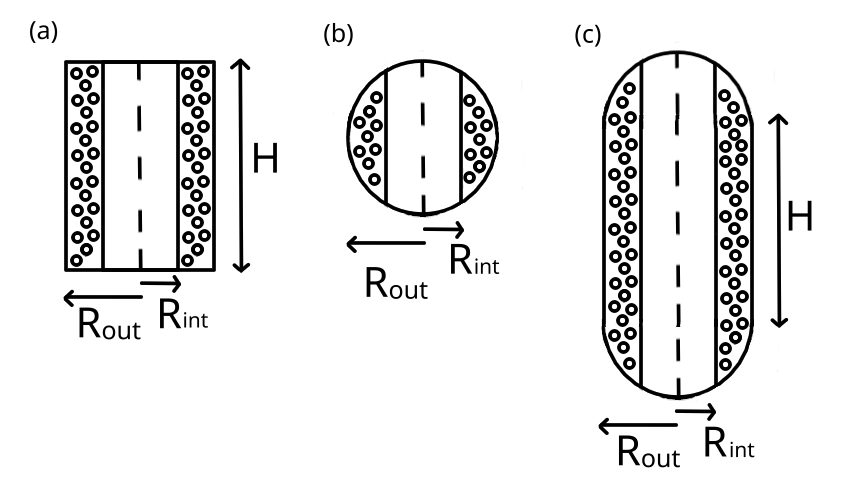
\includegraphics[width=0.7\textwidth]{analitical_geometries.png}
    \caption{Geometries that will be studied: (a) is a simple cylindrical capsid, (b) is a spherical capsid and (c) is a capped cylindrical capsid.}
    \label{fig:shapes}
\end{figure}

To compute the force, we will need to express the following quantities (see the equations below) as a function of $d_s$, $\rho_{pack}$, and $p$, which is the percentage of DNA that have been packed. These quantities can be expressed as a function of $R_{int}$ but it hides the dependency in $d_s$. Thus, we also express $R_{int}$ in terms of the variables $d_s$, $\rho_{pack}$, and $p$.

\subsection{Cylindrical capsid}

For the cylindrical capsid, the starting point is $h(R) = H$.
We deduce:
\begin{eqnarray}
    \int_{R_{int}}^{R_{out}} H 2 \pi R dr &=& \frac{d_s^2 \sqrt{3}}{2}L \\
    R_{int} &=& R_{out} \sqrt{1 - \frac{\sqrt{3}d_s^2L}{2 \pi H R_{out}^2}} \\
    \rho_{pack} &=& \frac{d_s^2 \sqrt{3} L}{2} \frac{1}{\pi h R_{out}^2} \\
    \int_{R_{int}}^{R_{out}} dR \frac{h(R)}{R} & = & -\frac{H}{2} \ln \left( 1-\rho_{pack}\right) \\
    A & = &\frac{\xi_p k_B T}{R_{out}^2} \left[ \frac{1}{ \left( 1 - \rho_{pack} p\right)} - \frac{\ln \left( 1-\rho_{pack}p \right) }{\rho_{pack} p} \right] \\
    G_{bend} &=& \frac{2 \pi k_B T H}{\sqrt{3} d_s^2} \ln \left( \frac{R_{out}}{R_{int}} \right) \\
    G_{charge} &=& L \sqrt{3} \left( c^2 + c d_s \right) \exp \left( \frac{-d_s}{c} \right)
\end{eqnarray}

Now to compute the force during the packing, we need to vary $p$ from 0 to 1. For each value of $p$ we compute $d_s$ (\ref{eq:cylds}). We can deduce the expression of the force via (\ref{eq:cylF}):
\begin{equation}
    0 = \sqrt{3} F_0 \exp \left( \frac{-d_s}{c} \right) - \frac{\xi_p k_B T}{R_{out}^2 d_s^2} \left[ \frac{1}{ \left( 1 - \rho_{pack} p\right)} - \frac{\ln \left( 1-\rho_{pack}p \right) }{\rho_{pack} p} \right] 
    \label{eq:cylds}
\end{equation}

\begin{equation}
    F_{pack} = \frac{2 \pi \xi_p k_B T}{2 R_{out}^2 \left( 1 - \frac{d_s^2 \sqrt{3} L}{2} \frac{1}{\pi H R_{out}^2}\right) } + F_0 \sqrt{3} \left( c^2 + cd_s \right) \exp \left( \frac{-d_s}{c} \right) \\
    \label{eq:cylF}
\end{equation}

We were able to implement these expressions numerically and make plots that are qualitatively similar to the plot presented in \cite{purohit2003}. Here we have considered that $L$ is the total length of the DNA strand, which means that when it is not fully packed, one should replace $L$ by $L\times p$ (this is true in all the above expressions).

\begin{figure}
    \centering
    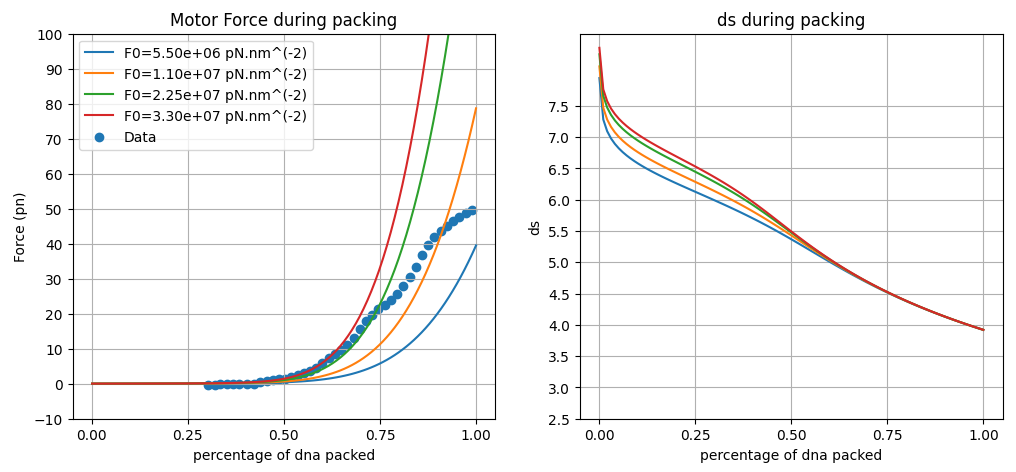
\includegraphics[width=0.9\textwidth]{Plot_ofTheForce_Cyl.png}
    \caption{We implemented these expressions in python. For each step, we set the parameter $p$ (percentage of DNA packed) determine $d_s$ via a the routine \url{scipy.optimize.root()}. We used the \url{'lm'} (Levenberg-Marquart) method (other method where not achieving to converge). Then, usind $d_s$ and $p$ one can compute the force. The parameters we used are : $k_B=1.380.10^{-23}JK^{-1}$, $T=310 K$, $R_{out} = 47 nm$, $h = 37.9 nm$, $ \xi_p = 25 nm$, $L = 3*6.584e3 nm$, $c_0 = 0.27 nm$ (close to \cite{purohit2003})}
    \label{fig:dseqcyl}
\end{figure}

We observe an evolution of $d_s$ that seems pseudo-exponential around $0$. This is because, at first, the strands will minimize their energy by being packed as far away from each other as possible, but will very quickly pack closer to each other to maximize their bending radius. Thus moving to the next regime we observe. Then the decrease is linear with the packing percentage. There is a trade off between the bending and the repulsion energy.

We also observe a slight change of regime in the evolution of $d_s$ between $p \in \left[5\%,\;45\%\right]$ where the trajectory of $d_s$ is affected by $F_0$, and $p \in \left[45\%,\;100\%\right]$ where the trajectory of $d_s$ is independent (and smilingly in continuity with the trajectory found at small $F_0$). We suppose that for small packing percentages ($p \in \left[5\%,\;45\%\right]$) the repulsion energy ($G_{charge}$ dependent in $F0$) has a significant impact, whereas for large packing percentages ($p \in \left[45\%,\;100\%\right]$) the geometrical properties of the capsid dominates the determination of $d_s$. This can be qualitatively understood by the fact that for high packing percentages, smaller and smaller bend radius occur. Finally we observe that our model for the force properly describe the evolution of the packing force for $F0=2.25.10^7pN.nm^{-2}$ for packing percentages $p \leq 75\%$. For packing percentages greater than $75\%$ our model doesn't describe the inflection of the force.

\begin{figure}
    \centering
    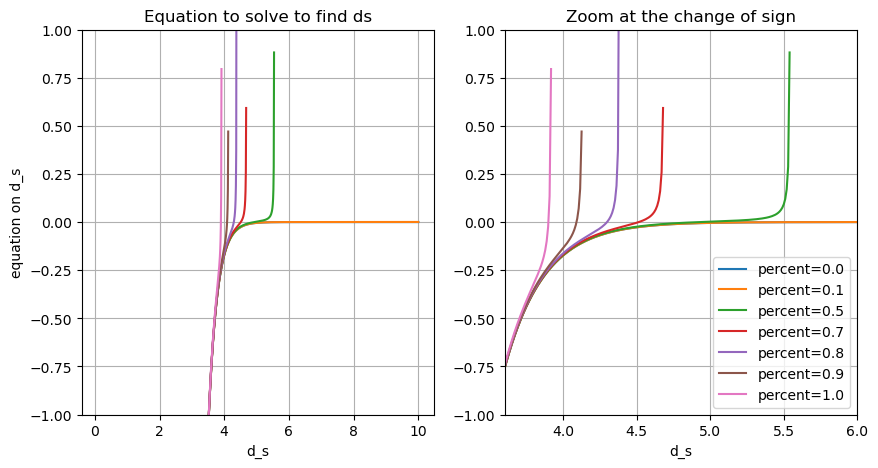
\includegraphics[width=0.9\textwidth]{Fig_Equation_cyl.png}
    \caption{Here is the illustration of the function we have to find the zero (see equation (\ref{eq:cylds})). This function is very steep close to zero.}
    \label{fig:equation-cylinder}
\end{figure}

We see in fig. \ref{fig:equation-cylinder} some sample of the equation (\ref{eq:cylds}). The divergence is provoked when $R_{int} = 0$. This corresponds to the fact that $d_s$ will have a maximal value before the length of DNA cannot fit in the capsid anymore. We observe that for higher packing percentage (previously shown to be $p \in \left[45\%,\;100\%\right]$ the inflexion comes before the solution (crossing with the x axis) whereas for low packing percentage (previously shown to be $p \in \left[0\%,\;45\%\right]$) the inflexion comes after the solution. This is another way to understand the absence of dependence of $d_s$ relative to $F0$ that has been remarked previously, as the inflexion only depend on the geometrical properties of the capsid and not on the repulsion energy.

\begin{figure}
    \centering
    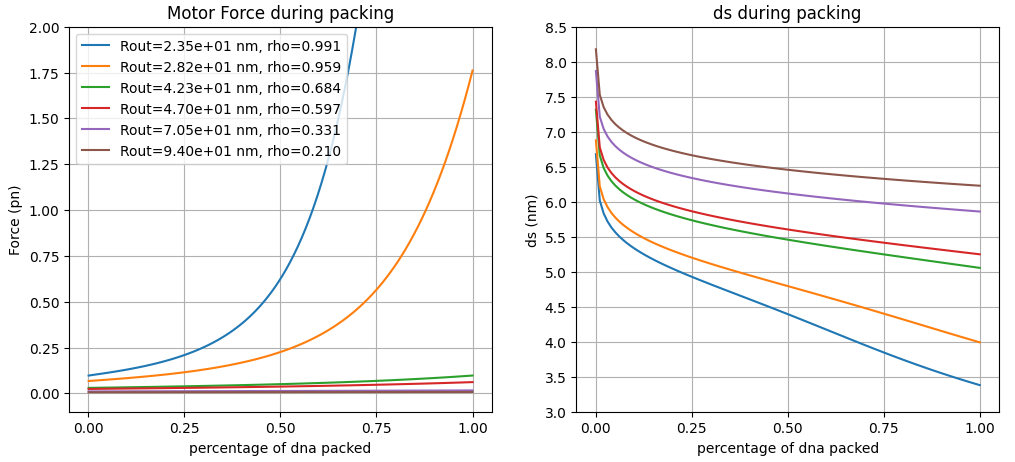
\includegraphics[width=0.8\textwidth]{Fig_Cylinder_FR.png}
    \caption{The evolution of the motor force during packing varies depending on the outer radius of the capsid. In the legend we have plotted as \url{rho} the packing ratio once the DNA has been fully packed ($p=1$). We see that for small packing ratio, the force remains small and the strands remains distant from one-another. We used the same parameters as in figure (\ref{fig:dseqcyl}) but $F_0 = 2.710^5 pN.nm^{-2}$ and $R_{out}\;$ is varying.}
    \label{fig:cylinder-fr}
\end{figure}

In fig. \ref{fig:cylinder-fr} we plot the motor force and $d_s$ for different capsid diameter ($R_{out}$). We observe that $d_s$ is smaller for smaller $R_{out}$ as the geometrical constrain implies that for the smaller capsid the DNA has to be packed in a more compact way. This in turn causes the motor force to be greater as the repulsion force is stronger. This can be understand qualitatively, as packing a strand of wool into a small container would be harder and harder the smaller the container gets (and thus the more densely packed the wool must have to be - i.e. the smallest the $d_s$ would have to get).


\subsection{Spherical capsid}

We can do the same analysis for a spherical capsid.
\begin{eqnarray}
    h(R) &=& 2 R_{out} \sqrt{1 - \frac{R^2}{R_{out}^2}}\\
    R_{int} &=& \left(1 - \left( \frac{d_s^2 L \sqrt{3}}{2 \frac{4\pi}{3} R_{out}^3} \right) ^{\frac{2}{3}}\right)^{\frac{1}{2}} R_{out} \\
    \rho_{pack} &=& \frac{\frac{\sqrt{3}}{2} d_s^2 L}{\frac{4}{3} \pi R_{int}^3} \\
    \int_{R_{int}}^{R_{out}} dR \frac{h(R)}{R} & = & -2 R_{out} \left[ \ln \left( \left( 1 - \rho_{pack}^{2/3}\right)^{-1/2} - \frac{\rho_{pack}^{1/3}}{\sqrt{ \left(1 - \rho_{pack}^{2/3}\right)}} \right) + \rho_{pack}^{1/3} \right] \\
    \int_{R_{int}}^{R_{out}} dR h(R) R &=& \frac{2}{3} R_{out}^3 \left( 1 - \frac{R_{int}^2}{R_{out}^2} \right)^{3/2} \\
    A &=& \frac{\xi_{p} k_B T }{R_{out}^2 \left( 1 - \rho_{pack}^{2/3} \right)} - \frac{3 \xi_p k_B T}{2 R_{out}^2} \left[ \frac{ \ln \left\{ \left(  1 - \rho_{pack}^{2/3} \right)^{-1/2} - \frac{\rho_{pack}^{1/3}}{\sqrt{ \left(1 - \rho_{pack}^{2/3}\right)}} \right\} + \rho_{pack}^{1/3}}{\rho_{pack}} \right] \\
    G_{bend} &=& \frac{-4 \pi \xi_p k_B T R_{out}}{\sqrt{3} d_s^2} \left[ \ln \left\{ \left( 1 - \rho_{pack}^{2/3} \right)^{-1/2} - \rho^{1/3} \left( 1 - \rho_{pack}^{2/3} \right)^{-1/2} \right\} + \rho_{pack}^{1/3} \right] \\
    F_{pack} &=& \frac{ \xi_p k_B T}{2 R_{out}^2 \left( 1 - \rho_{pack}^{2/3} \right) } + F_0 \sqrt{3} \left( c^2 + c d_s \right) \exp \left( \frac{-ds}{c} \right)
\end{eqnarray}

We have also implemented the equation that defines the $d_s$ of the spherical capsid numerically. The situation is more completed than for the cylindrical capsid. We find back the result of the previous section that from high packing percentage, $d_s$ is in fact determine only by the divergence of the equation which represent the maximum value of $d_s$. In this context, the repulsion between the strand and the geometry drives the system. We could also plot the force of the motor for different values of $F_0$ and the evolution $d_s$ for different value of $F_0$. One might be puzzled by the fact $d_s$ does not seem to depend on $F_0$ contrarily to what was obtained in figure (\ref{fig:cylinder-fr}). This is not really coherent with \cite{purohit2003} (see figure 2). We have state here that in fact the equation strongly sensitive to the choice of the parameters like $\xi_p$, $L_{dna}$, $F_0$ and $T$ we tried to use reasonable values building upon the literature (see the legend of figure (\ref{fig:cylinder-fr})). But the articles does not always state exactly all the parameters used for the plots (in particular $\xi_p$ which is stated to be '$\sim 50nm$'.

\begin{figure}[H]
    \centering
    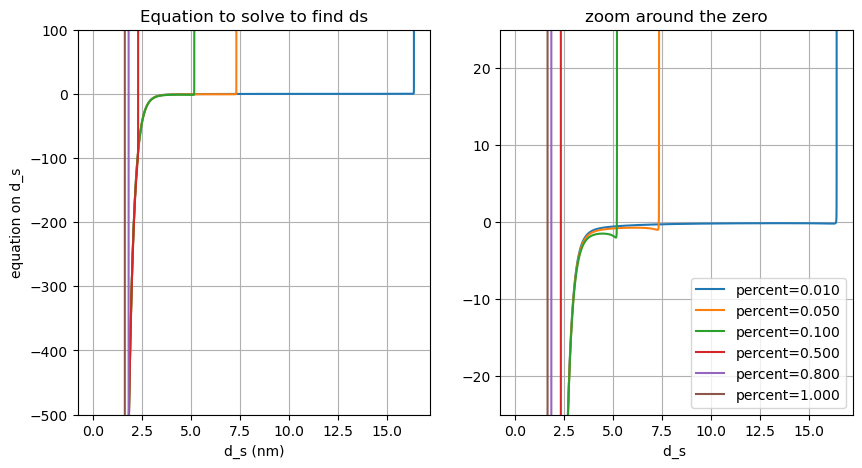
\includegraphics[width=0.9\textwidth]{Fig_Eq_sphere.png}
    \caption{The solution of $d_s$ that minimizes $G_{tot}$ is given by the zero of this function. This could be optain numerically via Levenbergh-Marquart method (like for the cylinder). However the function is so steep that this procedure will be very unstable numerically. Here the full proble is that the function is very steep close to its zero, and for small packing is very steep and very flat close to the zero. This cause both Newton-like and besectrice-like methods are not suitable.}
    \label{fig:eq-ds-sphere}
\end{figure}

\begin{figure}[H]
    \centering
    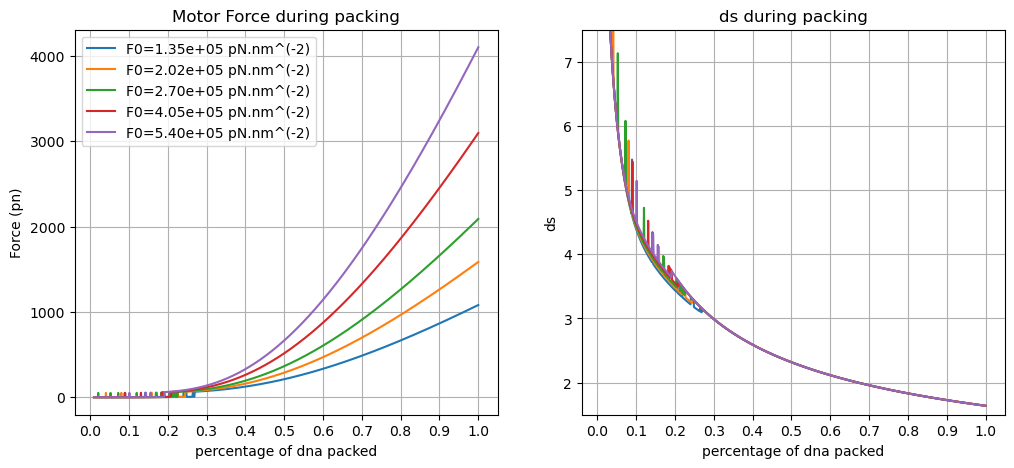
\includegraphics[width=0.9\textwidth]{Fig_ds_sphere.png}
    \caption{Force and evolution of $d_s$ as a function of the packing percentage in spherical geometry. We qualitatively recover the expected behaviour. There some spikes in the curve that only come from the numerical instability we have mentioned in figure (\ref{fig:eq-ds-sphere}).}
    \label{fig:force-sphere}
\end{figure}




\subsection{Capped cylindrical capsid}

We will now do the same analysis as in the previous section, but using a different geometry:

\begin{eqnarray}
    h(R) &=& H + 2Rout \sqrt{1 - \frac{R^2}{R_{out}^2}} \\
    \rho_{pack} &=& \frac{ \frac{4}{3}\pi R_{out}^3 \left( 1 - \frac{R_{int}^2}{R_{out}^2} \right)^{3/2} + \pi H R_{out}^2 \left( 1 - \frac{R_{int}^2}{R_{out}^2} \right) }{ \frac{4}{3} \pi R_{out}^3 + \pi H R_{out}^2 } \\
    G_{bend} & = & \frac{\pi k_B T \xi_p}{3 d_s^2} \left[ H \ln \left( \frac{R_{out}}{R_{int}} \right)  + 2R_{out} \ln \left( \frac{\sqrt{R_{out}^2 - R_{int}^2} + R_{out}}{R_{int}} \right) - 2 R_{out} \sqrt{\left( 1 - \frac{R_{int}^2}{R_{out}^2} \right)} \right] \\
    \frac{\sqrt{3}d_s^2}{2} L & = & \pi H R_{out}^2 \left( 1 - \frac{R_{int}^2}{R_{out}^2} \right) + \frac{4\pi}{3} R_{out}^3 \left( 1 - \frac{R_{int}^2}{R_{out}^2} \right)^\frac{3}{2} \\
    A &=& \frac{\xi_p k_B T}{R_{int}^2} + \frac{\xi_p k_B T}{2} \frac{ H \ln \left\{ \left( \frac{R_{out}}{R_{int}} - R_{out}\right) - \sqrt{ 1 - \frac{R_{int}^2}{R_{out}^2}} \right\} - \ln \left\{ \frac{R_{out}}{R_{int}} \right\} - \sqrt{\frac{R_{out}^2}{R_{int}^2}-1}}{\frac{4\pi}{3} R_{out}^3 \left( 1 - \frac{R_{int}^2}{R_{out}^2}\right)^{3/2} + \pi H R_{out}^2 \left( 1 - \frac{R_{int}^2}{R_{out}^2} \right) }
\end{eqnarray}

This very last expression could in principle be used to express $R_{int}$. It is doable analytically with help of a formal calculus program like Wolfram. But the expression obtained are so cumbersome that we will not even try to present them here. Expressing everything in terms of $\rho_{pack}$ seems hopeless.

In the impossibility of doing a numerical analysis, we can qualitatively say that the capped cylindrical capsid has two limits: for $R_{out} \gg H$ we end up with a capsid that can be considered spherical. In the opposite limit, for $H \gg R_{out}$ we end up with a capsid that will be dominated by its thin cylindrical body, and can thus be analysed in this limit.

\newpage
\section{Conclusion}

We were able, through a physical description of the DNA packing dynamics and analytical computation, to describe the different contributions to the energy cost to pack DNA. We were then capable of using these computations to numerically obtain results for the simpler cylindrical capsid geometry, and get a qualitative understanding of these results, which we could carry over to the other capsid geometries that we were unable to numerically analyze. We were also able to separate the packing process between two regimes where different contributions would determine the inter-strand spacing. We were, however, unable to explain the inflection observed in the real packing force as our model's packing force has a continuous exponential growth in the force with the packing percentage. This discrepancy was also observed in \cite{purohit2003, phillips2005}. Moreover, we did not find any article that was able to properly model this inflection. This could be because, as shown in \cite{comoli2008}, the actual packing isn't as simple as we assumed. In this paper it has been shown that the packing transition from a somewhat random packing occupying the whole capsid volume for low packing percentage, to an ordered phase for higher packing percentage.

\clearpage
\FloatBarrier
\printbibliography[
    heading=bibintoc,
    title={References}]
\clearpage
\FloatBarrier

\section*{Appendix}

\subsection*{Details of the computations of section 2}

Length of DNA in the capsid.
\begin{eqnarray}
    L & = & \int_{0}^{L} ds \\
    &=& \int_{R_{int}} ^{R_{out}} 2 \pi R \frac{2 N(R)}{\sqrt{3} d_s} dR \\
    &=& \frac{4 \pi}{\sqrt{3} d_s^2} \int_{R_{int}}^{R_{out}} R h(R) dR
    \label{eq:Ldef}
\end{eqnarray}


\subsection*{Minimization of $G$ \label{sec:Gmin}}

The conformation that DNA will take at steady state is the one corresponding to $d_s$ minimal. We thus have to minimize $G_{tot}$. Let us recall the expression :

\begin{eqnarray*}
    G_{tot} &=& \frac{2\pi \xi_p k_B T}{\sqrt{3} d_s^2} \int_{R_{int}}^{R_{out}} \frac{h(R)}{R} dR + L\sqrt{3} F_0 \left(c^2+cd_s \right) \exp{\left(\frac{-d_s}{c}\right)}
\end{eqnarray*}

We have to take the total derivative of this expression, in $d_s$ when $L$ is constant.
The part on the right of the plus sign, containing the electric repulsion between the strands leads to:
\begin{eqnarray}
    \frac{d G_{charge}}{d d_s} &=& - L \sqrt{3} F_0 d_s \exp{\left(\frac{-d_s}{c}\right)}
    \label{eq:deriv_gcharge}
\end{eqnarray}
Then we have to compute the derivative of the left side of the "$+$" sign. We have to take care that we must not derivate the L but we have to take the derivativ of the integral term which depends implicitly on $d_s$ via $R_{int}$.

Let us first derive some intermediary relation that will show up to be very usefull afterwards.
First let us express the volume of DNA inside the capsid.
\begin{eqnarray}
    \int_{R_{int}}^{R_{out}} 2 \pi R h\left( R \right) dR  &=& \frac{d_s^2 \sqrt{3}}{2} L
    \label{eq:L}
\end{eqnarray}
\begin{eqnarray*}
    \frac{d}{d R_{int}} \int_{R_{int}}^{R_{out}} 2 \pi R h\left( R \right) dR &=& - 2 \pi R_{int} h \left( R_{int} \right) \\
\end{eqnarray*}
\begin{eqnarray}
    \frac{d}{d R_{int}} \int_{R_{int}}^{R_{out}} R h\left( R \right) dR &=& \frac{d_s \sqrt{3} L}{2 \pi} \frac{d d_s}{d R_{int}}
    \label{eq:deriv_1}
\end{eqnarray}

 We use equation (\ref{eq:deriv_1}) to express:
 \begin{equation}
     \frac{d R_{int}}{d d_s} = \frac{-d_s \sqrt{3} L}{2 \pi R_{int} h \left( R_{int} \right)}
     \label{eq:derivativ_rint}
 \end{equation}
We deduce from equations (\ref{eq:derivativ_rint}) that:
\begin{eqnarray}
    \frac{d}{d d_s} \int_{R_{int}}^{R_{out}} dR \frac{h(R)}{R} &=&  \frac{\sqrt{3}L}{2\pi R_{int}^2}
\end{eqnarray}
We can reintroduce this expression in $ G_{bend} $ we have:
\begin{eqnarray}
    \frac{d G}{d d_s} &=& \frac{-2\pi \xi_p k_B T}{\sqrt{3} d_s^3} \int_{R_{int}}^{R_{out}} dR \frac{h(R)}{R} + \frac{k_B T L}{\sqrt{3} R_{int}^2}
    \label{eq:deriv_gbend}
\end{eqnarray}

We can put equations (\ref{eq:deriv_gcharge}, \ref{eq:deriv_gbend}). 
\begin{eqnarray*}
    \frac{d G_{tot}}{d d_s} &=& \frac{\xi_p k_B T}{d_s R_{int}^2} L - \frac{2 \pi \xi_p k_B T}{\sqrt{3} d_s^3} \int_{R_{int}}^{R_{out}} dR \frac{h(R)}{R} - L \sqrt{3} F_0 d_s \exp{ \left( \frac{-d_s}{c} \right)}
\end{eqnarray*}

\begin{eqnarray}
    \sqrt{3}F_0 \exp{ \left( \frac{-d_s}{c} \right)} &=& \frac{\xi_p k_B T}{d_s^2 R_{int}^2 } - \frac{2 \pi \xi_p k_B T}{\sqrt{3} d_s^4} \frac{\int_{R_{int}}^{R_{out}} dR \frac{h(R)}{R}}{L} 
    \label{eq:deriv_ds}
\end{eqnarray}

Using the expression of equation (\ref{eq:L}) we have the expression:
\begin{eqnarray}
    \sqrt{3} F_0 \exp{ \left( \frac{-d_s}{c} \right) } &=& \frac{\xi_p k_B T}{d_s^2 R_{int}^2} - \frac{\xi_p k_B T}{d_s^2} \frac{\int_{R_{int}}^{R_{out}} \frac{h(R)}{R} dR}{\int_{R_{int}}^{R_{out}} R h(R) dR} 
\end{eqnarray}

\subsection*{Computation of the general form of the force \label{sec:appenForce}}

In this appendix we drive the expression (\ref{eq:F}). We compute the derivativ of G in L assuming $d_s$ constant. This assumption is valid, because the variation $d d_s$ associated to $dL$ is of higher order. This is not trivial to prove that but it is a reasonable assumption given the shape of the equation of $d_s$ (\ref{eq:deriv_ds_final}).

\begin{eqnarray}
    \frac{d G_{tot}}{d L} &=& \frac{2 \pi k_B T \xi_p}{\sqrt{3} d_s^2} \left( - \frac{h(R_{int})}{R_{int}} \right) \frac{d R_{int}}{d L} + F_0 \sqrt{3} \left( c^2 + c d_s \right) \exp{ \left( \frac{-d_s}{c} \right) }
    \label{eq:F_appendix}
\end{eqnarray}

To compute $\frac{d R_{int}}{d L} $ do as in equation (\ref{eq:L}, \ref{eq:derivativ_rint}) but this time we derive by $L$ keeping $d_s$ constant.
\begin{eqnarray*}
    -R_{int} h(R_{int}) &=& \frac{d_s^2 \sqrt{3}}{4 \pi} \frac{ d L}{d R_{int}} \\
    \frac{d R_{int}}{dL} &=& \frac{ - d_s^2 \sqrt{3} }{ 4 \pi R_{int} h(R_{int}) }
\end{eqnarray*}
Reintroducing this result in (\ref{eq:F_appendix}) we obtain (\ref{eq:F}).

\subsection*{Computation of the force for different geometries}


\subsubsection*{Cylindric capsid}

1. Derivation of the force:

\begin{eqnarray*}
    F_{pack} & = & \frac{\partial G_{tot}}{\partial L} = (\frac{\partial G_{charge}}{\partial L} + \frac{\partial R_{int}}{\partial L} \frac{\partial G_{bend}}{\partial R_{int}}) \\
    F_{pack} & = & 3 G_{el}(d_s) + \left( \frac{\partial L}{\partial R_{int}} \right)^{-1} \frac{\partial G_{bend}}{\partial R_{int}} \\
    \frac{\partial L^{cylinder}}{\partial R_{int}} & = & -\frac{4 \pi }{\sqrt{3}d_s^2} H R_{int} \\
    \frac{\partial G_{bend}^{cylinder}}{\partial R_{int}} & = & - \frac{2\pi \xi_p k_B T}{\sqrt{3}d_s^2} \frac{H}{R_{int}}  \\
F_{pack}^{cylinder} & = & 3 G_{el}(d_s) +  \frac{\xi_pk_B T}{2R_{int}^2} = \sqrt{3}F_0(c^2 + cd_s)\exp(-\frac{d_s}{c}) + \frac{\xi_pk_BT}{2(R_{out}^2 - \frac{\sqrt{3}d_s^2L}{2\pi H})}
\end{eqnarray*}

2. Derivation of the optimal inter-strand spacing:

Using the general equation (\ref{eq:L}), we obtain the following condition for $d_s$:
\begin{eqnarray*}
\sqrt{3}F_0 \exp{ \left( \frac{-d_s}{c} \right)} &=& \frac{\xi_p k_B T}{d_s^2 R_{int}^2 } - \frac{2 G_{bend}^{cylinder}}{Ld_s^2} \\
\sqrt{3}F_0 \exp{ \left( \frac{-d_s}{c} \right)} &=& \frac{\xi_p k_B T}{d_s^2 R_{int}^2 } - \frac{2\xi_p k_B T}{d_s^2}\frac{\ln(\frac{R_{out}}{R_{int}})}{R_{out}^2 - R_{int}^2}
\end{eqnarray*}

\subsubsection*{Spherical capsid}
1. Derivation of the force:
\begin{eqnarray*}
 \frac{\partial G_{charge}^{sphere}}{\partial L} & = &  \sqrt{3}F_0(c^2 + cd_s)\exp(-\frac{d_s}{c}) \\
 \frac{\partial G_{bend}^{sphere}}{\partial L} & = & \left( \frac{\partial L}{\partial R_{int}} \right)^{-1} \frac{\partial G_{bend}^{sphere}}{\partial R_{int}} \\
 \left( \frac{\partial L}{\partial R_{int}}\right)^{-1}  & = & -\frac{\sqrt{3}d_s^2}{8\pi R_{int}}\frac{1}{\sqrt{R_{out}^2 - R_{int}^2}} \\
 \frac{\partial G_{bend}^{sphere}}{\partial R_{int}} & = & \frac{4\pi\xi_pk_BT}{\sqrt{3}d_s}[\frac{R_{int}}{\sqrt{R_{out}^2 - R_{int}^2}} - \frac{R_{out}^2}{R_{int}\sqrt{R_{out}^2 - R_{int}^2}}] = -\frac{4\pi\xi_pk_BT}{\sqrt{3}d_s} \frac{R_{out}^2 - R_{int}^2}{R_{int}\sqrt{R_{out}^2 - R_{int}^2}}  \\
 \Rightarrow  \frac{\partial G_{bend}^{sphere}}{\partial L} & = & \frac{\xi_pk_BT}{2R_{int}^2} =\frac{\xi_pk_BT}{2(R_{out}^2 - (\frac{3\sqrt{3}d_s^2L}{8\pi})^\frac23)}
\end{eqnarray*}
where we used the equation relating the internal radius $R_{int} = \sqrt{R_{out}^2 - (\frac{3\sqrt{3}d_s^2L}{8\pi})^\frac23}$ to the packaged length $L$.

The force is thus:
\begin{eqnarray*}
    F_{pack}^{sphere} = \frac{\partial G_{tot}^{sphere}}{\partial L}= \sqrt{3}F_0(c^2 + cd_s)\exp(-\frac{d_s}{c}) + \frac{\xi_pk_BT}{2(R_{out}^2 - (\frac{3\sqrt{3}d_s^2L}{8\pi})^\frac23)}
\end{eqnarray*}

2. Derivation of the optimal inter-strand spacing:

Using the general equation (\ref{eq:deriv_ds_final}), we obtain the following condition for $d_s$:
\begin{eqnarray*}
\sqrt{3}F_0 \exp{ \left( \frac{-d_s}{c} \right)} &=& \frac{\xi_p k_B T}{d_s^2 R_{int}^2 } - \frac{2 G_{bend}^{sphere}}{Ld_s^2} \\
\sqrt{3}F_0 \exp{ \left( \frac{-d_s}{c} \right)} &=& \frac{\xi_p k_B T}{d_s^2 R_{int}^2 } - \frac{3\xi_p k_B T}{d_s^2}\bigg[\frac{1}{R_{out}^2 - R_{int}^2} + \frac{R_{out}}{^(R_{out}^2 - R_{int}^2)^\frac32}ln\bigg(\frac{R_{out} - \sqrt{R_{out}^2 - R_{int}^2}}{R_{int}}\bigg) \bigg]  
\end{eqnarray*}
\end{document}
